\documentclass{birkjour}

\usepackage{tikz}
\usepackage{graphicx}
\usepackage{hyperref}

\newtheorem{thm}{Theorem}[section]
\newtheorem{cor}[thm]{Corollary}
\newtheorem{lem}[thm]{Lemma}
\newtheorem{prop}[thm]{Proposition}
\theoremstyle{definition}
\newtheorem{defn}[thm]{Definition}
\theoremstyle{remark}
\newtheorem{rem}[thm]{Remark}
\newtheorem*{ex}{Example}
\numberwithin{equation}{section}

\newcommand{\R}{\mathbb{R}}
\newcommand{\B}{\mathbb{B}}
\newcommand{\G}{\mathbb{G}}
\newcommand{\V}{\mathbb{V}}
\newcommand{\gd}{\dot{g}}
\newcommand{\gh}{\hat{g}}
\newcommand{\Gd}{\dot{G}}
\newcommand{\Gh}{\hat{G}}
\newcommand{\nvai}{\infty}
\newcommand{\nvao}{o}
\newcommand{\grade}{\mbox{grade}}

\received{August 25, 2013} \accepted{October 14, 2013}

\begin{document}


\title{The Mother Minkowski Algebra of Order $m$}

\author{Spencer T. Parkin}
\address{102 W. 500 S., \\
Salt Lake City, UT  84101} \email{spencerparkin@outlook.com}

%\subjclass{Primary 14J70; Secondary 14J29}

%\date{Augest 25, 2013}

\dedicatory{To my dear wife Melinda.}

\begin{abstract}
It is found that all polynomials of up to degree $m$
have an encoding as $m$-vectors in a geometric algebra referred
to as the Mother Minkowski algebra of order $m$.
It is then shown that all conformal transformations may be
applied to these $m$-vectors, the results of which, when converted
back into polynomial form, give us the transformed surfaces in terms
of the zero sets of the original and final polynomials.
\end{abstract}

\maketitle

\section{Motivation}

Before presenting the Mother Minkowski algebra of order $m$, we lead up to it here with
some background and motivation.\footnote{In all equations to follow, we let the
outer product take precedence over the inner product, and the geometric product
take precedence over the inner and outer products.  The inner product used in this
paper is the Hestenes inner product.  All polynomials and geometric algebras are assumed
to be defined over the field $\R$ of real numbers.}
We begin by recalling that an algebraic set is any 
subset of an $n$-dimensional euclidean space $\R^n$ that is also the zero set of one
or more polynomials, each in $n$ independent variables.  Given a geometric algebra $\G$, we can represent such sets
using blades $B\in\G$ as the set of all points $x\in\R^n$ such that
\begin{equation*}
p(x)\cdot B=0,
\end{equation*}
where $p:\R^n\to\V$ maps points in $\R^n$ to a vector space $\V$ generating
our geometric algebra $\G$.  Though not necessary, $\R^n$ is often embedded in $\V$;
but regardless of this, the function $p$ is necessarily defined in such a way that the expression
$p(x)\cdot B$ is a polynomial in the vector components of $x$ when $B\in\V$.

Letting $\B$ denote the set of all blades found in $\G$,
and letting $P(\R^n)$ denote the power set of $\R^n$,
we will find it useful to define the mapping $\gd:\B\to P(\R^n)$ as
\begin{equation}\label{equ_gd}
\gd(B) = \{x\in\R^n|p(x)\cdot B=0\}.
\end{equation}
To see that $\gd(B)$ is an algebraic set, we first observe that when $B\in\V$,
$\gd(B)$ is the zero set of a polynomial in the vector components of $x$.
Secondly, we observe that if $\bigwedge_{i=1}^k b_i$ is a factorization
of the $k$-blade $B$, each $b_i$ being in $\V$, then
\begin{equation}\label{equ_expand_p_dot_B}
p(x)\cdot B = -\sum_{i=1}^k (-1)^i (p(x)\cdot b_i)B_i,
\end{equation}
where each $B_i$ is given by
\begin{equation*}
B_i = \bigwedge_{\substack{j=1\\j\neq i}}^k b_j,
\end{equation*}
and therefore, since $\{B_i\}_{i=1}^k$ is a linearly independent set, we have
\begin{equation*}
\gd(B) = \bigcap_{i=1}^k \gd(b_i).
\end{equation*}

This method of representing algebraic sets using blades of a geometric algebra presents
some interesting properties.  To begin, if $A,B\in\B$ are blades with $A\wedge B\neq 0$,
then
\begin{equation*}
\gd(A)\cap\gd(B)=\gd(A\wedge B).
\end{equation*}
In this way, the outer product serves to take the intersection of two surfaces.  But we can also
look at the outer product in a different light as an operator that takes at least the union
of its two given surfaces.  To see this, we must consider an alternative interpretation
of blades $B\in\B$ as being representative algebraic sets.  Defining $\gh:\B\to P(\R^n)$ as
\begin{equation}\label{equ_gh}
\gh(B)=\{x\in\R^n|p(x)\wedge B=0\},
\end{equation}
we see that $\gh(B)=\gd(BI)$, where $I$ is the unit pseudo-scalar of $\G$, showing
that the image of $\gh$, like $\gd$, consists of algebraic sets.
Under this new interpretation, we find that for blades $A,B\in\B$, we have
\begin{equation*}
\gh(A)\cup\gh(B)\subseteq\gh(A\wedge B).
\end{equation*}
Exactly what surface we get from $A\wedge B$ in terms of $\gh$ can
be deduced by considering the surface $(A\wedge B)I$ in terms of $\gd$.

It is often useful to alternate between the interpretations provided by $\gd$ and $\gh$.
For example, while the intersection of two surfaces having no real intersection
may be perceived as an imaginary
surface, it is equally useful, if not more so, to switch from the $\gd$ interpretation to that of $\gh$,
the result of doing so being a real surface having geometric significance to the situation at hand.

What's further a benefit of using blades to represent surfaces is that of the many transformations
applicable to such geometries through the use of outermorphisms; in particular,
outermorphisms $f:\B\to\B$ of the form
\begin{equation*}
f(B) = VBV^{-1},
\end{equation*}
where $V$ is a versor of $\G$.  Given such a function, we wish to
compare $\gd(B)$ with $\gd(f(B))$.  Interestingly, to understand
the latter in terms of the former, we need only understand the mapping $h:\R^n\to\R^n$,
if any, induced by $V$ through $p$ as being each point $x\in\R^n$ mapped to a point
$y\in\R^n$ satisfying the condition
\begin{equation}\label{equ_induce_mapping}
V^{-1}p(x)V=\lambda p(y),
\end{equation}
$\lambda$ being some non-zero scalar in $\R$.
This is, of course, only a well defined mapping, provided that for every point $x\in\R^n$, there exists
such a point $y\in\R^n$, and that it is unique.
Assuming that $V$ and $p$ collectively meet these requirements, and so do indeed induce
such a mapping $h:\R^n\to\R^n$, we can show that
\begin{equation*}
\gd(f(B)) = h^{-1}(\gd(B)).
\end{equation*}
Notice that by the symmetry
of equation \eqref{equ_induce_mapping}, any argument that can be
used to show that $h$ is a well defined
mapping can also be used to show that $h^{-1}$ exists.
We now need only show that
\begin{equation*}
\gd(VBV^{-1})=\{x\in\R^n|V^{-1}p(x)V\cdot B=0\}.
\end{equation*}
To this end, we begin by factoring the $k$-blade $B$ as $\bigwedge_{i=1}^k b_i$.
Then, by substituting $V^{-1}p(x)V$ for $p(x)$ in equation \eqref{equ_expand_p_dot_B},
we see that
\begin{equation*}
V^{-1}p(x)V\cdot B=0
\end{equation*}
if and only if for all integers $i\in[1,k]$, we have
\begin{equation*}
0=V^{-1}p(x)V\cdot b_i=p(x)\cdot Vb_iV^{-1},
\end{equation*}
since the set of $k$ $(k-1)$-blades $\{B_i\}_{i=1}^k$ is a linearly
independent set.  Then, by applying equation $\eqref{equ_expand_p_dot_B}$ again
to obtain
\begin{equation*}
p(x)\cdot VBV^{-1} = -\sum_{i=1}^k(-1)^i(p(x)\cdot Vb_iV^{-1})VB_iV^{-1},
\end{equation*}
we see that
for all integers $i\in[1,k]$, we have $p(x)\cdot Vb_iV^{-1}=0$
if and only if $p(x)\cdot VBV^{-1}=0$, because the set $\{VB_iV^{-1}\}_{i=1}^k$ is
also linearly independent, which linear independence follows from that of the
set $\{B_i\}_{i=1}^k$.
It follows that $V^{-1}p(x)V\cdot B=0$ if and only if $p(x)\cdot VBV^{-1}=0$,
which is what we wanted to show.

\section{The Mother Minkowski Algebra of Order $m$}

Up to this point, we have kept the definition of the function $p$, and the signature of the
geometric algebra over which it is defined,
open to speculation, because the set of all possibilities for $p$, in terms of the types of geometry
we can consequently do, remains an open question.  What might be the most interesting and significant
definition of $p$ thus far proposed is found in \cite{Hestenes01} and given by
\begin{equation*}
p(x)=\nvao + x + \frac{1}{2}x^2\nvai.
\end{equation*}
Here, the vector space $\V$ is generated by the set
of basis vectors $\{\nvao,\nvai\}\cup\{e_i\}_{i=1}^n$,
where the set of $n$ euclidean vectors $\{e_i\}_{i=1}^n$ span
$\R^n$ as an orthonormal basis for that space, and the
vectors $\nvao$ and $\nvai$ are the null vectors representing the
points at origin and infinity, respectively.  Being null, we have $\nvao\cdot\nvao=\nvai\cdot\nvai=0$.
These basis vectors share the peculiar relationship $\nvai\cdot\nvao=\nvao\cdot\nvai=-1$.  The geometric
algebra generated by $\V$ is called a Minkowski algebra, and the resulting model of
geometry imposed upon this algebra by $p$ using functions \eqref{equ_gd} and \eqref{equ_gh}
is known as the conformal model of geometric algebra.  It has been shown in
\cite{Hestenes01,LiRockwood01,Dorst07} that
the versors of $\G$ generated by $\V$ induce the set of all conformal transformations through $p$.
The induced mappings are well defined and invertible.

Building upon the ideas presented in \cite{DoranHestenes93}, (specifically,
those surrounding the idea of what is referred to in \cite{DoranHestenes93}
as ``the mother algebra''), we will now consider
a new model of geometry based upon a geometric algebra $\G$
generated by a vector space $\V$ described in set builder notation as
\begin{equation*}
\V = \left\{\left.\sum_{i=1}^m v_i\right|v_i\in\V_i\right\},
\end{equation*}
where for each vector space $\V_i$, the geometric algebra $\G_i$ generated by $\V_i$
is a Minkowski algebra.  For all $i\neq j$, if $a\in\V_i$
and $b\in\V_j$, we have $a\cdot b=0$.  We will refer to the geometric algebra $\G$
generated by this vector space $\V$ as the Mother Minkowski algebra of order $m$.

Letting $\B$ denote the set
of all blades taken from $\G$, we now define the function $\Gd:\B\to P(\R^n)$ as
\begin{equation}\label{equ_Gd}
\Gd(B) = \left\{x\in\R^n\left|\bigwedge_{i=1}^m p_i(x)\cdot B=0\right\}\right.,
\end{equation}
where we define $p_i:\R^n\to\V_i$ as
\begin{equation}\label{equ_p_i}
p_i(x) = \nvao_i + x_i + \frac{1}{2}x_i^2\nvai_i,
\end{equation}
where $\nvao_i,\nvai_i\in\V_i$ are the familiar null vectors in the $i^{th}$ Minkownski sub-aglebra,
and where $x_i$ denotes the embedding
of $x$ in the $n$-dimensional euclidean sub-space of $\V_i$.  If more precision is needed here,
we can let $\B_i$ denote the set of all blades generated by $\V_i$,
let $\R_i^n$ denote the $n$-dimensional euclidean sub-space of $\V_i$, and then
work exclusively in $\R_1^n$ by defining an outermorphism that takes any blade in $\B_1$
to its corresponding blade in $\B_i$.  The function $p_i$ can then be defined in terms
of this outermorphism.  Interestingly, an explicit formula for this outermorphism can be found and carried through
all of the equations we'll present in the remainder of this paper, but there is no need to
formally introduce it, because the equations still go through in its absence; nor would we want to,
because it would just make the math less readable.  Nevertheless, if the reader is
interested, this outermorphism is given in the appendix.

In this paper we are going to limit our attention
to those blades $B\in\B$ having factorizations involving a representative from each $\B_i$,
which is to say that for all integers $i\in[1,m]$, there exists a non-zero vector $v\in\V_i$ such that $v\wedge B=0$.
Doing so, we write the blade $B$ as
\begin{equation}\label{equ_B_factored}
B = \bigwedge_{i=1}^m B_i,
\end{equation}
where each blade $B_i$ is in $\B_i$, and then see that
\begin{equation}\label{equ_exp_def}
\bigwedge_{i=1}^m p_i(x)\cdot B = (-1)^k\bigwedge_{i=1}^m p_i(x)\cdot B_i,
\end{equation}
where the integer $k$ is given by
\begin{equation}\label{equ_k}
k=\sum_{i=1}^m\sum_{j=1}^{m-i}\grade(B_j),
\end{equation}
letting the nested sum be zero in the case that $i=m$.
Then, subscripting equation \eqref{equ_gd} as
\begin{equation*}
\gd_i(B_i) = \{x\in\R^n|p_i(x)\cdot B_i=0\},
\end{equation*}
what we now find is that by equation \eqref{equ_exp_def}, we have
\begin{equation*}
\Gd(B) = \bigcup_{i=1}^m\gd_i(B_i).
\end{equation*}
This shows that we can represent any union of up to $m$ surfaces taken from the conformal model,
(let $B_i=\nvai_i$ to fill any remaining and unused blade factors),
but if we extend our function $\Gd$ to the set of all $m$-vectors, we can do even better.
To see why, we need only show that any monomial in up to $n$ variables and at most
degree $m$ can be represented by the expression on the right-hand side of equation \eqref{equ_exp_def}.
The $n$ variables are taken from the components of the point $x\in\R^n$.
Letting each $B_i$ be a vector in $\V_i$, the expression becomes
\begin{equation}\label{equ_monomial}
(-1)^k\prod_{i=1}^m p_i(x)\cdot B_i,
\end{equation}
with the integer $k$ becoming
\begin{equation}\label{equ_tri_numb}
k = \frac{m(m-1)}{2},
\end{equation}
the $(m-1)^{th}$ triangle number, since for all integers $j\in[1,m]$, we have $\grade(B_j)=1$ in
equation \eqref{equ_k}.
It is clear now that for an appropriate choice of each vector $B_i$, we can formulate any
monomial in the components of $x$ using equation \eqref{equ_monomial}.  In
every such choice, notice that we may let $B_i\cdot\nvai_i=0$.
Letting $B$ be a general $m$-vector, (which is not necessarily an $m$-blade),
we see now that the expression
that is the left-hand side of equation \eqref{equ_exp_def} represents
any polynomial of at most degree $m$
in the vector components of $x$, provided we have $B_i\cdot\nvai_i=0$
for all vector factors of any blade in $B$.
Of course, if this is not the case, what
we get is a polynomial of at most degree $2m$ by the squaring that
occures in equation \eqref{equ_p_i}, but we cannot represent all polynomials
of up to this degree.  If polynomials of a higher degree are needed, simply go to a
Mother Minkowski algebra of higher order.

As it turns out, the set of all polynomials of up to degree $m$ is closed under
the set of all planar reflections, and therefore the set of all
rigid body motions.  This set of polynomials, however, is not closed under the
set of all spherical inversions, and thefore the set of all
transversions and dilations.  This is where some of the polynomials of degrees
between $m$ and $2m$ come into play.

At this point an example may be in order to make things clearer.
Consider the Caylay cubic polynomial.
\begin{equation*}
-5(x^2y + x^2z + y^2x + y^2z + z^2x + z^2y) + 2(xy + xz + yz)
\end{equation*}
Realizing that the symbol $x$ in equation \eqref{equ_p_i} is reserved in denoting
a vector or point, another, although admittedly combersome way to express this polynomial, is as follows.
\begin{align*}
-5(x\cdot e_1)^2(x\cdot e_2) - 5(x\cdot e_1)^2(x\cdot e_3) -5(x\cdot e_2)^2(x\cdot e_1) \\
 -5 (x\cdot e_2)^2(x\cdot e_3) -5(x\cdot e_3)^2(x\cdot e_1) -5 (x\cdot e_3)^2(x\cdot e_2) \\
+ 2(x\cdot e_1)(x\cdot e_2) + 2(x\cdot e_1)(x\cdot e_3) + 2(x\cdot e_2)(x\cdot e_3)
\end{align*}
Here, we're letting $\{e_l\}_{l=1}^3$ be an orthonormal basis for $\R^3$.  Now let
$\{\nvao_i,\nvai_i\}\cup\{e_{l,i}\}_{l=1}^3$ be a basis for each $\V_i$ with a copy of $\R^3$
embedded in each of these.  The Caylay cubic polynomial can now be expressed by
equation \eqref{equ_exp_def}, if we let the blade $B$ be given by
\begin{align*}
B &= 5e_{1,1}\wedge e_{1,2}\wedge e_{2,3} + 5e_{1,1}\wedge e_{1,2}\wedge e_{3,3} + 5e_{2,1}\wedge e_{2,2}\wedge e_{1,3} \\
 &+ 5e_{2,1}\wedge e_{2,2}\wedge e_{3,3} + 5e_{3,1}\wedge e_{3,2}\wedge e_{1,3} + 5e_{3,1}\wedge e_{3,2}\wedge e_{2,3} \\
 & +2e_{1,1}\wedge e_{2,2}\wedge \nvai_{3} + 2e_{1,1}\wedge e_{3,2}\wedge \nvai_{3} + 2e_{2,1}\wedge e_{3,2}\wedge \nvai_{3},
\end{align*}
with the understanding that $x_i$ is given by
\begin{equation*}
x_i = (x\cdot e_1)e_{1,i} + (x\cdot e_2)e_{2,i} + (x\cdot e_3)e_{3,i}.
\end{equation*}
Here we're using a Mother Minkowski algebra of order 3.  Notice that in such higher order
algebras, and even this algebra itself, the encoding of the Caylay cubic is certainly not unique.
Another way to express this fact is to say that the function $\bigwedge_{i=1}^m p_i(x)$ does
not uniquely factor out of any given polynomial of at most degree $m$ in terms of the inner product.
Converting the trivector $B$ above back into the Caylay cubic polynomial is simply a matter
of expanding the expression $\bigwedge_{i=1}^3 p_i(x)\cdot B$.

When an $m$-degree polynomial surface equation is expressed in vector form, its conversion to an $m$-vector
can sometimes be given without reference to basis.

\section{Conformal Transformations}

While this new model certainly expands upon the set of all possible surfaces that may
be represented by
the conformal model, not all of the nice properties discussed in the motivating section
carry over very easily, if at all.
What we will show in this paper, however, is that all of the conformal transformations
are available in the new model.  It may be worth comparing this method
of applying such transformations to surfaces not native to the conformal model
to those found in \cite{Sobczyk12,Lasenby05}.

Letting $\{V_i\}_{i=1}^m$ be a set of $m$ versors, each $V_i$ taken from the
geometric algebra generated by $\V_i$, and each representing the same
conformal transformation, what we simply need to show is that
\begin{equation}\label{equ_conf_trans_poly}
\Gd(VBV^{-1}) = \left\{x\in\R^n\left|\bigwedge_{i=1}^m V_i^{-1}p_i(x)V_i\cdot B=0\right\}\right.,
\end{equation}
where the versor $V$ is given by
\begin{equation*}
V = \prod_{i=1}^m V_i.
\end{equation*}
It is clear that the right-hand side of equation \eqref{equ_conf_trans_poly} is
the surface $\Gd(B)$ having undergone the transformation represented by each $V_i$.
Our result will show that this is also the surface $\Gd(VBV^{-1})$.

To begin, we will first prove the validity of equation \eqref{equ_conf_trans_poly} for $m$-blades $B$ of $\G$,
and then after-word consider the more general case of $B$ as being a general $m$-vector.
We will therefore precede by factoring $B$ as we have in equation \eqref{equ_B_factored}
with each $B_i\in\V_i$.  We then have
\begin{align}
 & \bigwedge_{i=1}^m V_i^{-1}p_i(x)V_i\cdot B\label{equ_seq_start} \\
=\;& (-1)^k\prod_{i=1}^m V_i^{-1}p_i(x)V_i\cdot B_i\nonumber \\
=\;& (-1)^k\prod_{i=1}^m p_i(x)\cdot V_iB_iV_i^{-1}\nonumber \\
=\;&\bigwedge_{i=1}^m p_i(x)\cdot\bigwedge_{i=1}^m V_iB_iV_i^{-1}\label{equ_before_subscript_drop} \\
=\;&\bigwedge_{i=1}^m p_i(x)\cdot\bigwedge_{i=1}^m VB_iV^{-1}\label{equ_after_subscript_drop} \\
=\;&\bigwedge_{i=1}^m p_i(x)\cdot VBV^{-1},\label{equ_seq_stop}
\end{align}
where here, the integer $k$ is again given by equation \eqref{equ_tri_numb}.  The step taking us from
\eqref{equ_before_subscript_drop} to \eqref{equ_after_subscript_drop} deserves some explanation.
Removing the subscript $i$ from $V_i$ is done by inserting each of the factors $V_jV_j^{-1}=1$ with $j\neq i$
into the appropriate position, and then
commuting the $V_j^{-1}$ to the other side of $B_i$ into its appropriate position.  Finding the net change in sign
is an exercise in combinatorics, and ends up being
\begin{equation*}
(-1)^{m(m-1)}=1.
\end{equation*}

Returning now to equation \eqref{equ_conf_trans_poly} in the case that $B$ is a general $m$-vector, simply notice
that by the linearity of the inner, outer and
geometric products, the sequence of equalities equating \eqref{equ_seq_start} with \eqref{equ_seq_stop} remains valid.

This result suggests the following process of transforming a polynomial $f$ into another polynomial $f'$ by a conformal
transformation represented by a versor $V$.
\begin{center}
\begin{tikzpicture}[node distance=2cm, auto]
\node (f) {$f$};
\node (B) [above of=f] {$B$};
\node (VBV) [right of=B] {$VBV^{-1}$};
\node (fp) [below of=VBV] {$f'$};
\draw[->] (f) to node {} (B);
\draw[->] (B) to node {} (VBV);
\draw[->] (VBV) to node {} (fp);
\draw[->, dashed] (f) to node {} (fp);
\end{tikzpicture}
\end{center}
Here, the polynomial $f$ is converted into an $m$-vector $B$, the versor $V$ is applied to this $m$-vector
as the $m$-vector $VBV^{-1}$, which is in turn converted back into the polynomial $f'$.  The conversion
process is straightforward and can be easily handled by a computer algebra system, as well as that
of the computation of $VBV^{-1}$.

\begin{figure}
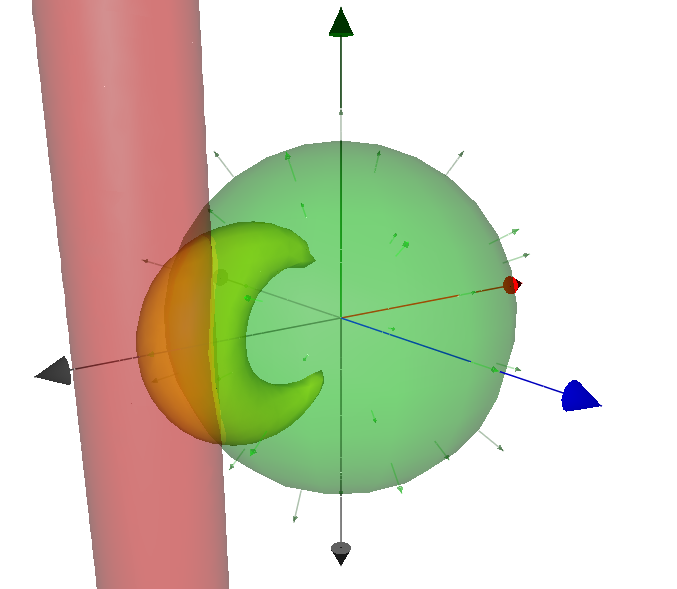
\includegraphics[scale=0.3]{InvertCylinderInSphere}
\caption{The inversion of a cylinder in a sphere.  A mesh generation algorithm was used to skin
the cylindrical and inverted surfaces.  The inverted surface mesh suffers where the curvature
of the object becomes extreme.}
\label{fig_invert_cylinder_in_sphere}
\end{figure}

Using the vector-based equations for quadric surfaces found in \cite{Miller87},
a piece of software\footnote{This software can be found at \url{https://github.com/spencerparkin/GAVisTool}.}
was written that implements the method given in this paper of
applying conformal transformations to polynomials.  This software was used
to generate Figure~\ref{fig_invert_cylinder_in_sphere}.  The input
polynomial, whose zero set is the cylindrical surface, was given by
\begin{equation*}
x^2 + z^2 + 14x + 45,
\end{equation*}
and the output polynomial, whose zero set is the inversion of the cylinder in the sphere,
came out to be
\begin{equation*}
\begin{split}
&28.8x^{2} + 11.2x^{3} + x^{4} + 11.2xy^{2} + 2x^{2}y^{2} + \\
&11.2xz^{2} + 2x^{2}z^{2} + y^{4} + 2y^{2}z^{2} + 28.8z^{2} + z^{4}.
\end{split}
\end{equation*}
The sphere was centered at origin and had a radius of 6.  The input polynomial
was not actualy fed to the software, but its conversion to a bivector was, because
it has an easy formulation when expressed in a vector-based form.  These formulations
are comparable to those of the conformal model for planes and spheres.

\section{Appendix}

As promised, the following function $f:\G_i\to\G_j$ is an outermorphism that can be used
to transform any element in $\G_i$ to its associated element in $\G_j$, provided $i\neq j$.
It is given by
\begin{equation*}
f(E) = S_1ES_1^{-1},
\end{equation*}
where $S_k$ is the element given by
\begin{equation*}
S_k = (1-(-1)^k e_{-,i}e_{-,j})(1+(-1)^k e_{+,i}e_{+,j})\prod_{l=1}^n(1+(-1)^k e_{l,i}e_{l,j}),
\end{equation*}
where $\{e_{l,i}\}_{l=1}^n$ and $\{e_{l,j}\}_{l=1}^n$ are the orthonormal bases for $\R_i^n$ and $R_j^n$, respectively,
and where $e_{-,i}$ and $e_{+,i}$ are each given by
\begin{align*}
e_{-,i} &= \frac{1}{2}(\nvai_i+\nvao_i),\\
e_{+,i} &= \frac{1}{2}(\nvai_i-\nvao_i).
\end{align*}
Take note that
\begin{equation*}
S_1^{-1} = \frac{S_0}{2^{n+2}}.
\end{equation*}
Although $S_k$ is not a versor, it can be shown that $f$ is an outermorphism.

For a vector $v_i\in\V_i$, to say that it's associated vector $v_j\in\V_j$ is $f(v_i)$ is to say
that for any integer $l\in[1,n]$, we have
\begin{equation*}
e_{l,i}\cdot v_i = e_{l,j}\cdot v_j,
\end{equation*}
as well as
\begin{align*}
\nvao_i\cdot v_i &= \nvao_j\cdot v_j,\\
\nvai_i\cdot v_i &= \nvai_j\cdot v_j.
\end{align*}
Notice that while $v_j=f(v_i)$, we have $v_i = -f(v_j)$.

\nocite{Milne12}
\begin{thebibliography}{9}

\bibitem{DoranHestenes93}%1.
C. Doran, D. Hestenes, F. Sommen and N. Van
Acker, {\it Lie groups as spin groups}. J. Math. Phys. {\bf 34}
 (1993), 8.

\bibitem{Dorst07}%2.
L. Dorst, D. Fontijne and S. Mann, {\it Geometric algebra for computer
science}. Morgan Kaufmann, 2007.

\bibitem{Hestenes01}%3.
D. Hestenes, {\it Old wine in new bottles: A new algebraic
framework for computational geometry}. Advances in Geometric
Algebra with Applications in Science and Engineering (2001), 1-14.

\bibitem{LiRockwood01} %4.
L. Hongbo, D. Hestenes and A. Rockwood, {\it Generalized homogeneous
coordinates for computational geometry}. Geometric Computing with
Clifford  Algebra Volume 24., Berlin Heidelberg, Springer-Verlag
(2001), 27-60.

\bibitem{Lasenby05}%5.
A. Lasenby, {\it Recent applications of conformal geometric
algebra}. IWMM 2004, LNCS 3519 Springer-Verlag (2005).

\bibitem{Miller87}%6.
J. Miller, {\it Geometric approaches to nonplanar quadric surface
intersection curves}. ACM Transactions on Graphics Vol. 6, No. 4, pp.
274-307.

\bibitem{[7]} J. Milne, {\it Algebraic geometry}. (v5.22), 2012, Available at
www.jmilne.org/math/, p. 260.

\bibitem{Sobczyk12}%8.
G. Sobczyk, {\it Conformal mappings in geometric algebra}. AMS Notices
Volume 59 (2012), 264-5.
\end{thebibliography}\end{document}

%\bibliographystyle{amsplain}
%\bibliography{Parkin_TheMotherMinkowskiAlgebraOfOrderM}

\end{document}
